% ---------------------------------------------------------------------------
% Part: The machinery.  Chapters follow sections/prog_groebner.tex.
% Draft 2026-11-06.  Every figure below is producer-reported unless the text
% names a VALIDATION.json with a passing validator report.
% ---------------------------------------------------------------------------

\chapter{Measuring an engine}\label{ch:engmeasure}

Chapter~\ref{sec:method} describes the instrument as it was built: the unit
$S$, sealed records, replay, isolation levels, the paired statistic and the
pricing band of \S\ref{sec:band}. Chapter~\ref{ch:matchedrho} describes how
the rho references inside that instrument were calibrated and corrected.
This chapter is about the other side of the same instrument: what it takes
to measure a decomposition engine, a linear-algebra stage or a whole
index-calculus pipeline so that the number survives a replay and a second
reader. Between 2 October and 5 November the harness changed its
accounting twice, its statistics once, and its notion of a passing audit
three times. Each change moved numbers that earlier chapters quote, and each
is stated here as what it is: a correction of the instrument, not an
improvement of any method.

Three distinctions run through this part of the treatise.
\begin{itemize}
\item A \emph{component speed-up} lowers the cost of one stage (a Macaulay
  build, an echelon, a lookup) with identical outputs. It is measured in
  the stage's own unit (word XORs, multiply-adds, instructions, stage
  wall time) and says nothing about the distance to rho until the stage
  is priced inside a whole solve.
\item An \emph{end-to-end change} moves the cold one-target $S$ of a
  complete pipeline, paired against the same pipeline before the change.
  It is an improvement under the programme's success criterion when it is
  verified and measured; it is a frontier move only when it also changes
  the order against the matched rho across the band of \S\ref{sec:band}.
\item An \emph{accounting change} moves a number without changing any
  algorithm: a counter that was not charged is charged, a reference is
  resized, an interval is recomputed. It is never an improvement, even
  when it moves the distance to rho in the method's favour.
\end{itemize}
Every result in Chapters~\ref{ch:engmeasure}--\ref{ch:instruments} carries
one of these three labels.

\section{What the calibration does and does not cover}\label{sec:em-calibration}

The calibration study of 2 October (\S\ref{sec:mr-calibration},
Table~\ref{tab:mr-calibration}) is the harness's only test against a
closed-form constant: seven generic methods reach their analytic constants
up to $r=2^{25.35}$ on prime curves and $2^{39}$ on Koblitz curves. For an
engine this has two consequences.
\begin{itemize}
\item The counted charge of every generic reference used below is
  calibrated in its own unit up to those sizes. A ratio of an
  index-calculus $S$ to a rho $S$ therefore has a calibrated denominator at
  toy size, and an uncalibrated one above $2^{39}$.
\item No index-calculus method has a closed-form constant, so no engine in
  this part is calibrated in the same sense. An engine's charge is
  checked only by replay (the same counts on a second run, host or
  instruction set) and by the independent recomputations named
  \texttt{VALIDATION.json} below; neither says that the unit is the right
  price for the work.
\end{itemize}
The second point is why the band of \S\ref{sec:band} exists: native work
(word XORs, conflicts, lookups, matrix entries) is priced at 0, 0.1 and
1~GAE per operation because no calibration can price it once for all
hosts, and two arms are ranked only where the order is the same at all
three prices.

\section{Accounting version 2}\label{sec:em-accounting}

PR~\#2465 (23 October) gave every frozen method identifier a versioned twin
and changed what each twin charges
(\art{research/ecbench_accounting_v2_20261023/REPORT.typ}; preregistered,
four dated amendments). The study's own first sentence classifies it: an
accounting and instrument correction, not an algorithmic improvement and
not a speed result. Its effect on the strong Koblitz reference is recorded
in \S\ref{sec:corr-engine}; its effect on engines is recorded here.
\begin{itemize}
\item \emph{The verification phase.} Every v2 identifier charges one final
  check $[d]G=Q$; \texttt{ic.large\_prime\_v2} also charges the membership
  check $[r]Q$. On matched (workload, round, seed) pairs the v2 total
  minus the frozen total equals the verification phase exactly on 40 of 40
  pairs for each of six generic methods and 16 of 16 for
  \texttt{ic.large\_prime}, and every other phase is equal. The
  preregistered outcome that the phase costs $1.5\log_2r$ failed for every
  record: it is the exact double-and-add count of the planted scalar
  (19 to 29~GAE here), so its size follows the scalar. The post hoc
  replacement held on 240 of 240.
\item \emph{What it costs.} On these toy curves a fixed 19--29~GAE sits on
  totals of 235--1{,}500~GAE, so v2 identifiers cost $1.7$--$8.8\%$ more
  $S$ (for example $1.022$ $[1.021,1.024]$ for \texttt{bsgs.textbook} and
  $1.0003$ for \texttt{ic.large\_prime}). The study states that this is a
  sizing statement for these curves and not for larger $r$, since one
  scalar multiplication is $O(\log r)$ against $O(\sqrt r)$.
\item \emph{No frozen count moved.} The same frozen-only specs run on the
  branch binary and on the main binary agree on every count field of
  504 of 504 matched records. Two committed sessions fail a replay
  identically on both binaries, in their root-finding and inherited-F4
  arms only (96 and 16 problems): a pre-existing condition, not caused by
  the change, that CI's \texttt{--replay 0} audit does not see.
\item \emph{The distance moves the other way.} The index-calculus arms of
  the committed claim specs are unchanged; their reference became cheaper.
  The best arm across the band, \texttt{ic-rootfind-m2}, reads
  $10.6$--$11.0\times$ the v2 strong reference at $n=13$ (against
  $2.0$--$2.3\times$ the frozen one) and $34$--$49\times$ at $n=19$
  (against $10$--$11\times$). The report states that the corrected
  reference makes the measured gap larger.
\end{itemize}
The v2 floor rule (\texttt{automorphisms/v2}) also counts six automorphisms
on $j=0$ and four on $j=1728$; under the first rule a cubic-automorphism
rho read $0.720$ $[0.591,0.867]$ of a floor computed with two automorphisms,
which is impossible for a correct floor. That correction belongs to the rho
side (Chapter~\ref{ch:matchedrho}); for engines its lesson is that a floor
is part of the instrument and is versioned with it.

\section{Statistics version 2: censoring and the wall statistic}\label{sec:em-stats}

PR~\#2442 replaced the comparison statistic; \S\ref{sec:mr-stats} gives the
interval widths, the coverage simulation and the censored-rho rows. Three
of its changes bear on engines specifically
(\art{research/ecbench_statistics_v2_20261105/README.md}; no new runs, the
old and new binaries run on the same committed records).
\begin{itemize}
\item \emph{Censored engine runs are rows.} An engine that times out or
  exhausts its budget now enters the ratio as a censored lower bound. On
  the yield sweep the two descent-SAT arms over strong rho move from
  $1.351$ (9 of 16 pairs) to $1.429$ $[1.241,1.646]$ with 7 censored, and
  from $1.892$ to $2.486$ $[1.442,4.288]$ with 4 censored; both are lower
  bounds. The point estimate over verified pairs is unchanged in every
  row, so the old binary and the new agree where both define a number.
\item \emph{Wall time per operation, not per solve.} The v1 headline wall
  statistic was the median per-pair solve-wall ratio, whose interval was
  often a single point. The v2 headline is the ratio of nanoseconds per
  GAE. The two answer different questions and can disagree in direction:
  on the yield sweep, \texttt{sub8-mitm} over strong rho reads $20.26$ as a
  median wall ratio and $0.627$ $[0.489,0.804]$ in ns per GAE, because the
  arm does $45\times$ the operations at a lower cost per operation. The
  descent-SAT arms read $5.1\cdot10^7$ and $8.8\cdot10^6$ ns per GAE: their
  solver work is unpriced, and the harness now flags them as upper bounds
  on that statistic.
\item \emph{The tail flag needs runs.} A heavy-tail flag (largest run
  above 25\% of an arm's total) fired on 71 of 71 table rows with four runs
  and on 6 of 6 with two: with $n$ runs the largest share is at least
  $1/n$, so at $n\le4$ the flag carries no information. The same PR made
  the threshold depend on $n$.
\end{itemize}
The engine-side lesson is the first item. A decomposition engine that
times out on a hard target is not cheaper on the targets it finished; a
comparison that drops it reads the engine as cheaper than it was. Every
engine ratio quoted from a session with censored runs before 5 November is
a lower bound on the engine's cost, and some (\texttt{ic-sub6-mitm}, $6.98\to
648$) were understated by two orders of magnitude.

\section{The allocator confound}\label{sec:em-allocator}

A runner change (PR~\#2455) reported its index-calculus online window
``about 15\% lower''. A preregistered study of the same day
(\art{research/ecbench_allocator_confound_20261023/REPORT.md}; ABBA order,
three scratch ablations) measured what the change did.
\begin{itemize}
\item \emph{Counts are identical.} Ten base-versus-variant session pairs
  match on every count-bearing field of every record (72 of 72 and 66 of 66
  per pair); a tampered copy is flagged by the same script.
\item \emph{The small-set arms' wall time collapses.} Eight rho, BSGS and
  kangaroo arms on a 20-bit prime curve read pooled medians of
  $5.26$--$6.77$\,ms on the merge-base binary and $0.137$--$0.330$\,ms on
  the PR binary, $18.4$--$38.8\times$ shorter; the index-calculus
  \texttt{ic-mitm} arm (about 1.9\,ms) does not move (ratio $1.03$).
\item \emph{The online window is not distinguished.} On the Koblitz $n=17$
  claim spec the IC online median moves from $127.1$ to $119.1\,\mu$s
  (ratio $1.067$; $1.135$ and $0.983$ by order). The ``15\% lower'' is not
  reproduced; the preregistered verdict is inconclusive.
\item \emph{Attribution.} Removing \texttt{malloc\_trim(0)} alone, or the
  new pre-solve \texttt{/proc} reads alone, leaves the PR binary fast;
  removing both returns every arm to the merge-base level ($0.75$--$1.05$).
  Either consolidates the allocator before the clock starts.
\end{itemize}
The study measured the distance to rho on the same claim spec, which no
binary changes: the band gives the IC arm $16.85$, $17.28$ and $21.16$
against the strong rho's $4.00$, $4.14$ and $5.36$ at $w=0,0.1,1$, so IC is
$4.21$, $4.17$ and $3.95\times$ the strong rho, and a plain signed-Frobenius
rho ($1.54$--$2.48$) is cheaper than both at this size because the strong
walk's set-up dominates at $r=2^{16}$. For engines the lesson is that wall
time on sub-millisecond solves measured the allocator; the PR's own grader
now refuses wall time below 1\,ms of solve.

\section{Sessions that cannot be cited in full}\label{sec:em-registries}

Committed sessions are evidence and are never edited. Two registries record
those that cannot pass the audit as committed
(\art{docs/ecbench/}).
\begin{itemize}
\item \emph{Incomplete sessions} (\art{docs/ecbench/INCOMPLETE_SESSIONS.tsv},
  since 18 October): four frozen scratch sessions of the $k=4$
  quartic studies, committed without spec and host capsules. Each row pins
  the SHA-256 of \texttt{session.json}, \texttt{plan.json} and
  \texttt{records.jsonl}; the CI audit reports them as incomplete
  evidence, never as audited passes, and fails if a byte changes or a
  capsule appears.
\item \emph{Defective sessions} (\art{docs/ecbench/DEFECTIVE_SESSIONS.md},
  one row, owner-approved 5 November): the interrupted timing smoke of the
  Curve25519 algebraic ladder. Its \texttt{session.json} claims 7 records
  and a stop at sequence 6, but \texttt{records.jsonl} holds sequences
  0--3, and the sealed records hash is that of the 4-line file, so the
  records were lost on the producer's host before sealing. Recovery from
  Git and from the S3 checkpoints found nothing. The row pins all five
  capsule hashes and the exact four problem checks
  (\texttt{record\_count}, \texttt{status\_counts}, \texttt{last\_seq},
  \texttt{stop}); the audit passes the row only if verify fails with
  exactly those checks. The session is citable as its four sealed records
  only (\S\ref{sec:c25519}).
\end{itemize}
A third class is reported but not fatal: a session whose audit receipt says
\texttt{records\_bound: false} (no whole-file hash binds its records, for
example a runner killed before finalisation) is listed as an unbound prefix,
not integrity-passed (\art{.github/scripts/ecbench-audit-sessions.sh}).

\section{The registry, inventoried}\label{sec:em-inventory}

By 1 November the harness exposed 79 top-level methods and 24 nested
algorithms behind them: 11 system solvers, 9 three-summand decomposition
(PDP3) engines and 4 prime Kummer-tower engines
(\art{research/ecbench_registry_optimization_20261101/README.md}). A native
audit (\texttt{ecbench optimize inventory} and \texttt{audit}) admits a
development roster of 114 specs covering 79 of 79 methods and 24 of 24
nested algorithms, with no structural errors or seed leakage.
\begin{itemize}
\item \emph{Execution coverage.} 38 fresh L0 sessions (1{,}095 records,
  1{,}042 verified outcomes) exercised 73 of 73 runnable native methods and
  every nested engine; 854 of 854 eligible deterministic measured replays
  reproduced with zero audit problems. Six entries are external CM wrappers
  without a hash-bound backend and are not executable.
\item \emph{A replay that found a defect.} The first pair-index F6 replay
  exposed an accounting-cache regression; resetting the cache at the
  independent-run boundary makes the corrected session reproduce 16 of 16.
\item \emph{What the count does not include.} A standalone $n=83$
  chained-$\Sem3$ lookup (\S\ref{sec:bo-n83}) and a \texttt{chained-x}
  decomposition oracle registered in \texttt{ic bench} are outside the
  79+24, because neither is ecbench-selectable; the README lists wiring and
  pricing them as a coverage gap, not an assumed result.
\end{itemize}
The inventory changes no distance. Its use is negative: an engine that is
in the registry has been run at least once under the same accounting as
rho, and an engine that is not has not.

\section{The end-to-end frontier refresh}\label{sec:em-frontier}

The refresh of 31 October and 1 November
(\art{research/ecbench_e2e_frontier_20261031/README.md},
\art{research/ecbench_e2e_frontier_20261031/REPORT.md})
bound the frontier to one source commit, inventoried every live method and
every nested engine, and prepared a 92-shard isolated campaign that did not
run (no checkpoint credential; the blocker is recorded). Its answer is a
boundary statement, with the domains kept apart as
Definition~\ref{def:domain} requires.
\begin{itemize}
\item \emph{Generic prime, random binary and medium Koblitz ladders are
  rho-led.} No admitted cold one-target index-calculus result in those
  panels is below its strongest matched reference. The closest markers are
  $2.28\times$ rho for inherited F4 on one tiny random-binary cell, $2.59\times$
  for the prime residual collector at 36 bits (\S\ref{sec:pg-residual}) and
  $3.43\times$ on Table~A's rule-v7 Koblitz ladder, whose rho reference
  was $0.57$--$0.85$ of the strong walk per step, so that figure understates
  the gap by about $1.7$--$2.0\times$ (\S\ref{sec:tablea},
  \S\ref{sec:kc-rho}); the report states that these are different studies
  and units, not entries of one table.
\item \emph{Engines on the current binary.} The pair-index F6 reduces
  inherited-F6 work to $0.2792$ $[0.246,0.317]$ and is still $139.30$
  $[85.48,227.02]\times$ strong rho end to end; the prime PKM F4, F5, F6 and
  enumeration engines are $4.62$--$5.03\times$ negation rho; the best
  matched $n=17$ system solver is wide FES/Gray code at $4.28\times$ strong
  rho. All are one-target L0 operation comparisons with unpriced work.
\item \emph{Historical engine counts are bound to their binary.} A fresh
  replay of the F4/F5/F6 cross-family sessions on the current binary
  reproduces 72 of 144 deterministic rows, while the optimised-rho session
  reproduces 720 of 720. The engine claims of Table~\ref{tab:prog_groebner-engineering}
  are therefore statements about the binary that produced them.
\item \emph{One restricted family is IC-led.} The plane-quartic attack on
  the GHS-weak family $E_0/\FF_{q^3}$ with $\#E_0=4\ell$ is below matched
  rho in its own comparison (\S\ref{sec:transfer}); the report keeps it out
  of the generic ranking because it is a different problem class.
\end{itemize}

\paragraph{The $n=29$ crossover is Frobenius-folded BSGS.} One panel does
cross below rho, and its classification is the instructive part
(\art{research/ecbench_generator_orbit_20261022/README.md}; protocol frozen
before data). The study measured an orbit-layout pair table and a
generator-orbit factor base on seven Koblitz curves ($n=13$--$37$). The
layout table finds the same relations as the lazy table on 960 of 960 run
pairs at $1.02$--$1.09\times$ lower cost; with the generator-orbit base and
stride the net gain over the lazy baseline is $1.26$--$3.20\times$, with the
order holding across the band: an end-to-end improvement over an
index-calculus baseline. At $n=29$ and one factor-base column the IC arm
reads $S=0.546$, $0.611$ and $1.196$ at $w=0,0.1,1$ against $1.569$ for
\texttt{rho-frob}, a paired ratio of $0.366$ $[0.241,0.523]$. The directory
carries a \texttt{VALIDATION.json} with a replay certificate and a passing
validator report (a validation-gate pass; no pcc claim, so an unverified
assertion under the 4 November rule), and its own scope statement says what
the crossing is.
\begin{itemize}
\item At one column the pipeline is a Frobenius-folded baby-step
  giant-step with a known generator-orbit column, not a factor base with
  unknown logarithms; in the language of \S\ref{sec:gf-collision} it has
  $F=0$.
\item The crossing rests on \texttt{rho-frob}'s fixed 133-GAE set-up at
  $\log_2r=15.4$. The gap to rho grows with $r$: $1.15\times$ at $n=31$,
  $1.93\times$ at $n=23$ and $3.89\times$ at $n=37$; at $n=17$, 23, 31 and
  37 \texttt{rho-frob} is ahead at every weight, at $n=13$ the pair is
  unresolved, and at $n=19$ the band cannot re-price the IC natives (no
  pinned calibration row).
\item In the validation file's like-for-like band, which prices the same
  native operation types on both arms, rho rises from $1.503$ to $1.58$ at
  $w=0.1$ while the IC arm reads $0.413$, $0.478$ and $1.063$; the crossing
  holds under that choice at this size and does not survive growth in $r$.
\end{itemize}
The refresh therefore keeps the panel as a fixed-set-up engineering
frontier and does not pool it with the uniform-target ladder; the 1
November current-binary snapshot reads the same cell at $0.4405$
$[0.363,0.534]$ of signed-Frobenius rho and calls it a holdout candidate,
not a family-level or leaderboard result. It is the clearest example in
the programme of a validated number below rho that is not an
index-calculus advance.

\section{The cost of the harness itself}\label{sec:em-overhead}

A measured child is a fresh \texttt{ecbench exec} process, so the harness's
own start-up sits inside every wall time it records. Two engineering
studies measured that share without changing any counted unit.
\begin{itemize}
\item \emph{Registry and alias parses}
  (\art{research/ecbench_child_overhead_20261024/README.md}; Callgrind
  instructions, frozen protocol). Before \#2184 every child parsed the whole
  4.7\,MB curve registry, about 190\,M instructions or 98\% of a rho or BSGS
  child; after it a \texttt{rho.negation} child runs $4.26$\,M instructions
  ($4.64$\,M on \texttt{main}).
  The index-calculus child had meanwhile grown a parse of the 2.8\,MB alias
  table to match one curve name against a 25-row calibration table: $169.47$\,M
  instructions on \texttt{main}, $9.86$\,M after the fix. Median spawn-to-exit
  wall time per child fell from $37.20$ to $2.92$\,ms after \#2184
  ($0.0786$ $[0.0769,0.0802]$); the alias fix's own wall ratio, $0.9910$
  $[0.9754,1.0083]$, is not distinguished.
\item \emph{Inversion in the default IC oracle}
  (\art{research/ecbench_ic_asm_euclid_20261103/README.md}). A 32-bit
  extended-Euclid inversion in x86-64 assembly lowered instructions per GAE
  of the default \texttt{mitm:negation\_folded=1} oracle from $537.0$ to
  $476.8$ ($-11.2\%$) and of the prime-batch arm from $427.2$ to $397.7$; the
  target had been a halving. Every counted field of every record is
  identical to \texttt{main}'s.
\end{itemize}
Neither changes an $S$. Both matter for the wall-time column: an
index-calculus child that spends most of its instructions finding its curve
name, or a rho child that spends 98\% parsing a registry, makes an
admitted wall-time ratio a ratio of start-up costs. This, with
\S\ref{sec:em-allocator}, is why wall time is admitted only above a minimum
solve length and with an A/A interval.

\section{What a measured engine result must carry}\label{sec:em-contract}

The corrections above add up to a contract that every result in the
following chapters is read against. An engine result is citable as a
component speed-up when it carries identical outputs on frozen inputs, a
same-binary A/A, a preregistered gate, and its own unit. It is citable as an
end-to-end change when, in addition, it is a sealed ecbench session (or an
equivalent native record) with every phase charged or explicitly unpriced,
censored runs kept, and a paired comparison against the pipeline it
replaces. It is citable against rho only when the rho arm is the strongest
available for the curve (Chapter~\ref{ch:matchedrho}), measured in the same
process and unit, and the order is stated per band weight. It is
\emph{validated} only where its directory names a \texttt{VALIDATION.json}
whose validator report passed; everything else in this part is a
producer-reported figure, which is how the text marks it.
\chapter{Boolean decision engines}\label{ch:boolean}

Over a binary field the decomposition oracle receives the Weil restriction
of a summation polynomial: a Boolean system in $N$ unknowns whose solutions
are the decompositions of one target over the factor base. The index
calculus needs a \emph{decision} (a witness or a proof that there is none), not a
Gr\"obner basis, and almost every target has none. Chapter~\ref{sec:groebner}
describes the four engine families and Table~\ref{tab:prog_groebner-engineering}
lists their headline engineering ratios. This chapter gives what that
chapter compresses: the generic Boolean search campaign that preceded the
algebraic engines, the gate methodology of the $\FF_2$ micro-studies and the
variants it refuted, the inherited-F4 rounds after 5 October, the F6-IC
engine's convergence to the meet-in-the-middle oracle, the crossbred and
SAT engines, and the $n=83$ engine campaign. One observation recurs: as an
engine is made faster on index-calculus systems it tends to turn into an
enumeration with a table, and the table is the generic oracle whose cost
Chapter~\ref{ch:genericfloor} bounds from below.

\section{Generic Boolean search, 22 September to 3 October}\label{sec:bo-generic}

Before the descended Semaev systems were fed to an algebraic engine, a
campaign of standalone studies measured complete generic Boolean solving on
generated public systems of up to 36 variables: exact specialisation,
affine propagation, fixed branch selection (most frequent variable, zero
first) and exhaustive search below a node cap, with node and resource limits
returning \textsc{unknown} and never \textsc{unsat}. None accepts a curve or
a target; every result is a component result on its own fixture
distribution. Each study froze its protocol, held out seeds, rotated arm
order, and compared a candidate against the \emph{pointwise fastest} of all
retained methods rather than against the method it replaced. Most
preregistered a universal $2\times$ gate (every size and family group with a
paired 95\% lower bound above 2), which almost nothing passed.
Table~\ref{tab:bo-generic} lists the outcomes.

\begin{table}[t]
\centering\small
\begin{tabularx}{\linewidth}{@{}>{\raggedright}p{0.27\linewidth}>{\raggedright}X>{\raggedright\arraybackslash}p{0.2\linewidth}@{}}
\toprule
Study & Result (paired, against the fastest retained method) & Verdict \\
\midrule
Packed direct construction & construction only: $3.48$--$4.53\times$ (primary), $3.55$--$4.90\times$ (confirmation) & passes $2\times$ on construction; no solve claim \\
Construction plus reduction & charging the full RREF, the staged path is $1.38$--$1.50\times$ faster at $n=36$ than either streaming candidate; candidates pass 0 of 9 & both rejected \\
Fixed quadratic state & $2.40$--$2.51\times$ on 9 of 9 primary comparisons; confirmation $2.10$--$2.55\times$, 7 of 9; 6{,}144 verified solves & engineering; same search tree \\
Packed residual coefficients & $1.56$--$1.67\times$ against the fastest of 8 methods, 18 of 18 lower bounds above 1; 5{,}832 observations on 72 systems & incremental gate passes; $2\times$ rejected \\
Linear tail ($W\cap L$ kernel) & $3.59\times$ $[3.57,3.62]$ on the large-active mixture; four small cells $0.964$--$0.975$ & guarded portfolio rejected \\
Whole-solve traces & degree-3 hybrid kernel slower than the flat kernel with identical traces; search-only often faster with more nodes; specialisation gain $1.04$--$1.14\times$ & $2\times$ rejected \\
Row-space transport & full-RREF paired ratios $0.199$--$2.667$ (3 of 18 groups); affine-tail $0.235$--$0.952$ (0 of 18) & rejected \\
Affine substitution, SIMD Gray & $16/18$ and $15/18$ groups above 2 & universal gate rejected \\
Sibling pivot-trace screen & 0 of 64 eligible $n\ge12$ branch pairs keep a replayable pivot trace & rejected at the structural gate \\
\bottomrule
\end{tabularx}
\caption[]{Generic Boolean search on generated systems, September--October.
All complete-solve timings, correctness pass on every row. Sources, top to
bottom: \art{research/boolean_packed_construction_20260922/},
\art{research/boolean_construction_reduction_20260922/},
\art{research/boolean_quadratic_state_20260923/},
\art{research/boolean_quadratic_frontier_20260923/},
\art{research/boolean_linear_tail_20260923/},
\art{research/boolean_solve_trace_20260923/},
\art{research/boolean_basis_transport_20260923/},
\art{research/boolean_affine_substitution_20260923/},
\art{research/boolean_pivot_screen_20261003/} (each \texttt{CONCLUSION.md}
or \texttt{README.md}).}
\label{tab:bo-generic}
\end{table}

Two results of this campaign shaped what followed. First, at 24 variables
the degree-3 Macaulay kernels were slower than plain search: on the packed
residual study's planted holdouts the flat kernel took $253.1$\,ms per solve,
the sparse-bucket kernel $1{,}050$\,ms and search-only $53.8$\,ms, against
$12.0$\,ms for packed residuals
(\art{research/boolean_quadratic_frontier_20260923/CONCLUSION.md}). On small
systems a closure that sees further is more expensive than a search that
looks less far. Second, every accepted gain was a faster representation of
the same search tree: node counts, logical counters and canonical trace
digests are identical across arms, so the campaign moved constants and
never an exponent. The lead atlas records the same reading for every
Boolean engine (\art{crypto-autoresearcher:knowledge/leads/ecdlp/ic-engine/LEAD-ICE-boolean-f4-f5-f6-engines.yaml}).

\section{The $\FF_2$ micro-studies and their gate}\label{sec:bo-gate}

About thirty matrix-F5 and Boolean F4 variants were tested between 26
September and 3 October against one fixture: the $n=24$, degree-4 complete
F5 call of a seven-case suite (\texttt{f5\_n24\_m24\_d4}), and the
\texttt{n20\_m30} Boolean F4 workload. The gate was the same in every study,
and it is why most variants failed.
\begin{itemize}
\item The protocol and an unmodified baseline build were committed before
  candidate code or timing; the candidate was opt-in and was removed again
  if it failed.
\item One release binary ran both arms. Each selected block had two
  warm-ups, five reference/reference A/A pairs and five alternating A/B
  pairs, 22 processes and all seven cases per process; the first isolated
  exact block per seed was selected before its timing was read.
\item Every arm had to match raw and canonical row fingerprints, rank,
  terms, columns, builder and criterion counts and reduction word
  operations on every case.
\item Ratios are medians of the five paired ratios, with exact
  $3{,}125$-resample bootstrap intervals; a candidate advanced only with a
  frozen one-thread complete-call ratio of at least $1.05$ and a lower
  bound above $1.02$, and no smaller case below its own A/A minimum.
\end{itemize}
Table~\ref{tab:bo-refuted} lists the refuted variants with the ratio that
refuted them; the accepted ones are in Table~\ref{tab:prog_groebner-engineering}.

\begin{table}[t]
\centering\small
\begin{tabularx}{\linewidth}{@{}>{\raggedright}p{0.3\linewidth}>{\raggedright}X>{\raggedright\arraybackslash}p{0.23\linewidth}@{}}
\toprule
Variant & Complete-call ratio (reference/candidate) & Why it failed \\
\midrule
AVX2 gather unpack & $0.9652$ $[0.9630,0.9874]$ (1 thread, Intel), $0.9140$ (2 threads, AMD) & slower \\
AVX2 nibble compaction & $0.912$ $(0.906$--$0.925)$ & slower \\
Nibble-subset unpack & $0.649$ $(0.646$--$0.650)$ & slower \\
AVX-512 unpack & new over prior $0.996$--$1.016$ & no gain \\
POPCNT unpack & $1.0005$ $(0.9944$--$1.0067)$ & below $1.05$ \\
Compact paired unpack & $0.9998$ $(0.9986$--$1.0045)$ & below $1.05$ \\
Bounds-free unpack & $1.004$, $0.982$ (ARM64 screen) & below $1.05$ \\
One-pass unpack & $0.992$, $0.953$ & below $1.05$ \\
x86-guarded direct unpack & $0.9984$ $(0.9927$--$1.0226)$ & below $1.05$ \\
Contiguous (flat) rows & $0.978$, $1.002$ & below $1.05$ \\
Byte-colex packing & $1.0229$--$1.0262$; build phase $1.46\times$ & below $1.05$ \\
Initial-density row order & $1.006$, $0.987$ & below $1.05$ \\
Bounded-weight pivots ($K=8,16$); stratified pivots & terms $0.964$--$0.984$ of reference (bounded) & structural gate (both) \\
Always-echelon output & large case $1.50$--$1.55$; \texttt{n12\_m12\_d4} $0.821$--$0.830$ & smaller-case regression \\
Fused row build, 4 threads & build $1.382$, complete call $0.865$ $(0.745$--$1.095)$ & 4-thread gate \\
Boolean F4 unsorted products & $0.857$, $0.876$ & slower \\
Boolean F4 degree-bucket queue & $0.993$--$1.008$ & below $1.05$ \\
Boolean F4 six-column tables & primary $1.074$; holdout \texttt{n20\_m20} $0.881$ & smaller-case regression \\
\bottomrule
\end{tabularx}
\caption[]{Refuted $\FF_2$ engine variants, 26 September--3 October:
complete F5 call (\texttt{n24\_m24\_d4}) unless marked F4
(\texttt{n20\_m30}), frozen seed unless a range is given. Each source is
\art{research/<study>/RESULT.md}: \texttt{f5\_avx2\_gather\_unpack\_20260929},
\texttt{f5\_avx2\_nibble\_unpack\_20260929},
\texttt{f5\_nibble\_subset\_unpack\_20260929},
\texttt{f5\_avx512\_unpack\_20260929}, \texttt{f5\_popcnt\_unpack\_20260929},
\texttt{f5\_compact\_unrolled\_unpack\_20260929},
\texttt{f5\_bounds\_free\_unpack\_20260930},
\texttt{f5\_one\_pass\_unpack\_20260929},
\texttt{f5\_x86\_guarded\_unpack\_20260930}, \texttt{f5\_flat\_rows\_20260929},
\texttt{f5\_byte\_colex\_20260930},
\texttt{f5\_initial\_density\_order\_20260929},
\texttt{f5\_bounded\_weight\_pivots\_20260930} and
\texttt{f5\_stratified\_weight\_pivots\_20260930},
\texttt{f5\_echelon\_20260927}, \texttt{f5\_row\_build\_20260928},
\texttt{boolean\_f4\_unsorted\_products\_20260926},
\texttt{boolean\_f4\_degree\_queue\_20260927},
\texttt{boolean\_f4\_wide\_tables\_20260926}.}
\label{tab:bo-refuted}
\end{table}

\paragraph{What passed, and its size.} The one complete-call result above
$2\times$ is the support cut at column 19: a CI recheck on the same four
seeds passed every cell, with one-thread medians of $3.006$--$3.049\times$
(lower bounds $2.970$--$3.024$) and two-thread medians of $2.415$--$2.476\times$,
the candidate's counted reduction XORs being $28.08$--$28.10\%$ of the
reference's (\art{research/f5_support_cut19_final_recheck_20261003/RESULT.md}).
The README calls it a recheck, not an independent second holdout. Its
predecessor, the support split, cut reduction word operations to $33.7\%$
but its ARM64 timings were non-promoting, with one seed's lower bound at
$0.966$ (\art{research/f5_support_split_call_20261002/RESULT.md}), and the
mainline rank port read $1.450\times$ with an interval of $0.582$--$1.664$
(\art{research/f5_mainline_port_20261002/RESULT.md}).

\paragraph{Defaults, 17 October to 29 October.} Three switches that had
passed their incremental gates on x86 CI were left opt-in because their
protocols tied a default change to the $2\times$ gate. A decision rule
committed before the deciding run made one of them a default: direct F5
packing ($1.006$--$2.173\times$ on every F5 cell); direct unpack stayed opt-in
at $0.986\times$ on one four-thread cell, and table reuse at $0.955\times$ on a
matrix-F4 cell, and with all three on the largest F5 cases ran
$1.11$--$1.27\times$ faster than the previous defaults
(\art{research/f5_gf2_defaults_20261017/README.md}; L0, round-to-round
variation up to $\pm25\%$). On GitHub's Arm runners (Neoverse-N2 and a
virtual Apple M1) every x86-chosen default stayed: the lazy rewrite with the
bit scatter, Arm's path before \#2043, takes $1.08$--$1.69\times$ more CPU on
Linux; turning gate-first F6-IC off costs $1.69$--$2.10\times$ on Linux and
$1.62$--$2.15\times$ on macOS; and no Gray-code table count beats four
(\art{research/arm64_f4_defaults_20261022/README.md}). The follow-up of 29
October tried four more candidates and landed none: a four-row
multiply-accumulate pass cut the $\FF_p$ kernels from 976\,M to 633\,M
instructions with no wall gain ($0.88$--$1.08$ per site), because the loop is
bound by reading pivot rows; a column-tiled parallel $B'$ build was
$0.87$--$1.02\times$ the control; and F5 direct unpack ``where it wins''
passed its rule on one output mode while identical code on the degree-3
cases read $1.087$ against $0.933$ across runs, a disagreement larger than
the effect, so it stayed opt-in
(\art{research/f4_f5_followups_20261029/README.md}).

\paragraph{Reading.} The campaign's own standard is the right one: a
stage gain is an engine result, the complete call is the unit that matters
for the oracle, and the oracle is a minor share of an index-calculus solve
whose relation phase is dominated by the number of targets tried. None of
these studies, accepted or refuted, changes a distance to rho.

\section{Inherited F4 after 5 October}\label{sec:bo-inherited}

Inherited F4 has been the default algebraic oracle since 22 September
(Chapter~\ref{sec:groebner}). Its later rounds were of four kinds.

\paragraph{Instruction rounds.} Two preregistered rounds lowered the machine
work behind the counted unit without moving the unit. The overhead round
ran $0.847\times$ the baseline's instructions on the confirmatory $m=19$
inputs (threshold $0.90$), with 48 of 48 frozen outputs identical; inherited
F4 went from about 120 to about 95 instructions per counted word XOR
(\art{research/inherited_f4_overhead_20261005/RESULT.md}). The remap round
read $0.923\times$ (threshold $0.97$; about 95 to 89 per word XOR) but was
superseded before merge by a more general word-wise rewrite on
\texttt{main} (\art{research/inherited_f4_remap_20261007/RESULT.md}). The
eager rewrite through shift runs then brought hosts without BMI2 onto the
eager path: $1.22$--$1.70\times$ lower median CPU on six of nine cells
against the bit scatter, and the two architectures charge the same units
again (\art{research/inherited_f4_eager_runs_20261016/README.md}). Because
an eager rewrite charges every kept row, it charges \emph{more} word XORs
than the lazy one while using less CPU: a reminder that word XORs are a
stage unit, not a cost.

\paragraph{A batching idea that lost.} Replaying one F4 trace on several
specialisations at once, after Demin's Groebner.jl tracer, was exact but
used $2.2$--$4.0\times$ more stage units than the sequential root and more
CPU (\art{research/lit2026_w5_lane_batched_f4_20261011/README.md}). The same
study found the gate-first order for F6-IC ($1.57$--$1.78\times$ lower stage
unit), which became a default after an x86 check on nine cells ($1.336$--$1.733\times$
fewer word XORs, 80 of 80 targets decided identically;
\art{research/f6_gate_first_x86_20261016/README.md}).

\paragraph{Online, against rho.} The first public-target panel (one
registered point, prepared 62-point base, three fixed process orders) put
F5 at a median $208.49\times$ ($181.29$--$223.86$) inherited F4's online time
and inherited F4 about $315\times$ slower than the rho reference online; both
engines spent over $99.9\%$ of the online window in \texttt{target\_PDP}
(\art{research/ic_solver_online_20261003/RESULT.md}). A capture defect (the
wrapper's \texttt{time} exited 1 on the sandboxed host) makes the panel
diagnostic only. Its useful datum is the split count: F5 used 2{,}546 splits
on the first, unsuccessful target attempt against inherited F4's 68, which
is why a matrix-kernel gain cannot be projected onto the online path.

\paragraph{The harvest default.} PR~\#1862 made the root linear-row harvest
the default; on the one workload a pricing bisect saw it raised counted word
XORs by about 7\%. A preregistered re-measure on five curves
(\art{research/f4_harvest_remeasure_20261024/README.md}; five sessions of 144
records, 144 of 144 replays identical, counts only) found that the sign
depends on size (Table~\ref{tab:bo-harvest}). The $m=2$ negative control
reads $1.0000$ on all five curves.

\begin{table}[t]
\centering\small
\begin{tabular}{@{}llrcrr@{}}
\toprule
Curve & $\dim V$ & default/off & 95\% interval & targets up/down & $S$/frozen strong rho, off$\to$default \\
\midrule
$n=11$, K1 & 4 & $1.0958$ & $[1.0940,1.0980]$ & 24/0 & $7.17\to7.86$ \\
$n=13$, K0 & 5 & $1.0699$ & $[1.0646,1.0759]$ & 24/0 & $36.9\to39.5$ \\
$n=17$, K1 & 6 & $0.9969$ & $[0.9955,0.9985]$ & 6/18 & $424.1\to422.8$ \\
$n=19$, K1 & 7 & $0.9593$ & $[0.9576,0.9611]$ & 0/24 & $1{,}248\to1{,}198$ \\
\bottomrule
\end{tabular}
\caption[]{Inherited F4 at $m=3$: total $S$ with the root linear-row harvest
on (the default since \#1862) over off, 24 paired public targets per curve.
At $n=19$ (K0) the word XORs are unpriced and $S$ is flat; priced at $0.1$
or 1~GAE the ratio is $0.9755$. Source:
\art{research/f4_harvest_remeasure_20261024/README.md}.}
\label{tab:bo-harvest}
\end{table}

\noindent The default is a regression at $n=11$ and 13 and a $4.1\%$
engineering gain at $n=19$; at $n=17$ the whole gain comes from a different
gate (\#1891's root-rank gate). Every priced F4 arm sits $7$ to $1{,}250$
times the frozen strong rho, and the harvest moves that by at most $10\%$. The
correction is listed in Chapter~\ref{ch:corrections}.

\paragraph{Determinism.} The cross-host drift of \S\ref{sec:corrections}
(item 6) was first searched for within one host: thread count, a second
process with new hash seeds and a replay under a different thread count
all gave byte-identical word counts on 48 of 48 rows
(\art{research/inherited_f4_replay_determinism_20261018/README.md}), which
excluded the within-host sources and left the instruction-set path, later
confirmed as the cause.

\paragraph{The priced distance.} With its word XORs priced, inherited F4 is
about $22$--$33\times$ the frozen strong rho at $n=13$, and the complete pair table
is $17$--$22\times$ cheaper than F4 on the same cells; the atlas records the
whole Boolean-engine line as \emph{closed, dominated} by the pair-table
oracle on Koblitz and random binary curves up to $n=31$, $m\le4$
(\art{crypto-autoresearcher:knowledge/leads/ecdlp/ic-engine/LEAD-ICE-boolean-f4-f5-f6-engines.yaml}).
A later diagnostic on a \texttt{chained-x} oracle read inherited F4 at
$24.71$, $144.09$ and $794.37\times$ matched rho at $m=2,3,4$ on Koblitz
$n=13$; matrix F5 cut matrix F4's work at $m=3$ to $0.6276$ and still cost
$16{,}296.76\times$ rho, and both $m=4$ matrix arms were censored
(\art{research/ecbench_registry_optimization_20261101/README.md},
\art{research/ecbench_e2e_frontier_20261031/REPORT.md}). The atlas also
records that on the $\Sem3$ chain F4 and F6-IC grow faster in $n$ than the
meet-in-the-middle floor at $m=3$ and $m=4$, with the slope-difference
interval above zero.

\section{F6-IC: from closure to lookup}\label{sec:bo-f6}

F6-IC adds to inherited F4 a factor-base domain gate and meet-in-the-middle
leaves (Chapter~\ref{sec:groebner}). Its record after 5 October is a single
argument in three steps.

\paragraph{Step 1: the closure is charged, and loses.} On the $E_0$ ladder
(eight public targets per size, 72 verified runs per arm and size, word XORs
counted but not charged, geometric additions charged) F6-IC's $S$ was
$54.75\times$ (37.81--84.22) the same-target rho at field degree $n=13$
(the source writes $m$ for the degree) and $2{,}091\times$ at $n=19$, against
inherited F4's $1.105$ and $1.582$; at $n=23$ the two IC arms were $2.72$ and
$2.09\times$, and at $n=31$ both hit the 3{,}600-second
cap on the first target, so the protocol reached no decision
(\art{research/f6_ic_ecbench_ladder_20261005/RESULT.md}). The frozen strong
rho of that ladder carried its set-up (\S\ref{sec:em-accounting}), and the
inherited-F4 figures are the unpriced lower bounds that
\S\ref{sec:corrections} (item 5) corrects.

\paragraph{Step 2: the time is in the matrix build, not the gate.} Online on
the prepared $n=17$ curve, rho was faster on both frozen public points:
rho/IC online $0.0219$--$0.0221$ on T1 and $0.000515$--$0.000530$ on T7
(\art{research/f6_ic_rho_online_gap_20261006/RESULT.md}). A nested profile of
T7 found the Macaulay stage at $81$--$84\%$ of target PDP for all three arms,
of which the matrix construction was $98.5\%$, and the F6 oracle callback at
$1.6$--$2.3\%$; eliminating every nanosecond inside the oracle would save
about $1.6\%$ of the online window
(\art{research/f6_ic_phase_profile_20261006/RESULT.md}).

\paragraph{Step 3: the few-candidate closure makes the algebra vanish.} On
5 November the gate was changed to run the exact one-fixed closure as soon
as a summand's assigned bits leave at most 64 base codes, deciding the whole
subtree; the change is now on by default
(\texttt{KIC\_F6\_FEW\_CANDIDATES=64}; \texttt{=0} is the same-binary
control) (\art{research/f6_few_candidates_20261105/README.md}; nine Koblitz
cells, $5\times3$ rounds, L0).
\begin{itemize}
\item Verdicts and indices are identical in both arms (80 target--engine
  pairs); F6-IC process CPU
  falls $2.67$--$10.29\times$ (median of five; worst round pairing at least
  $1.66$), word XORs $1.84$--$10.13\times$, and nodes from 204--1{,}049
  reductions per cell to 5--16. Inherited F4, with no gate, is unchanged
  ($0.87$--$1.05\times$ CPU).
\item The gate's pair lookups and group additions are \emph{identical} with
  and without the closure. On these cells the algebra was not ruling out a
  single candidate abscissa: F6-IC with the pair index was the pair-index
  meet-in-the-middle scan wrapped in Gr\"obner work.
\item The README states the conclusion, and marks it unverified: the change
  does not beat ecbench's \texttt{mitm} oracle, because in the limit it is
  that oracle.
\end{itemize}
Two companion items of the same study bound what remains. Re-reducing a
node's displaced rows (36--61 median per node, 7.9--24.5 pivots crossed per
row) by Four-Russians batching would spend about 32 row operations per pivot
on its tables, several times the roughly 1{,}500 row XORs per node it
replaces, so nothing was changed. A parallel split of one target's tree into
$2^k$ subtrees is $1.59$--$2.88\times$ faster in wall time on refuting cells
and $0.94$--$1.11\times$ on cells where most targets decompose, at
$1.12$--$1.49\times$ (refuting) and $2.67$--$2.86\times$ (decomposing) the counted
work, and stays opt-in because it changes the count.

On the current binary the pair-index F6 is at $0.2792$ of inherited F6 and
still $139.30\times$ strong rho (\S\ref{sec:em-frontier}). The F6 line is
therefore an engine that became a lookup, and a lookup is priced by
\S\ref{sec:gf-collision}.

\section{MutantXL closure as an engine}\label{sec:bo-mutantxl}

The closure instrument \texttt{dreg\_closure} (Chapter~\ref{ch:instruments})
is also a decision engine: MutantXL-style, it multiplies the fallen
lower-degree polynomials by variables and re-closes, and it refuted all 92
unsatisfiable draws of 23 cells at degree 3--4 where plain XL needed 5--7
(\S\ref{sec:binary}; \art{research/dreg_closure_mutantxl_20261016/RESULTS.md}).
As an engine its costs are those of a dense degree-4 closure: at
$(m,n,\ell)=(3,22,8)$ one branch has $124{,}314$ degree-4 columns, a scan
of 124--331\,s and a peak of 10.6\,GB
(\art{research/dreg_closure_guess_20261022/RESULTS.md}). At $(3,19,7)$ a
hybrid guess that restores degree 4 still costs $5.3\cdot10^{11}$ to
$1.5\cdot10^{12}$ word operations per draw
(\art{research/dreg_hybrid_guess_20261024/RESULTS.md}). The closure's value
is as an instrument that measures a degree, which is how
Chapter~\ref{ch:instruments} uses it; no study priced it as an oracle against
rho.

\section{Crossbred, exhaustive search and engine suites}\label{sec:bo-suites}

A matched engine suite (22 September) froze the contract every algebraic
engine is compared under: identical targets in one process, systems
fingerprinted, timeouts never read as \textsc{unsat}, units named, missing
values null (\art{research/ic_framework_engines_20260922/README.md}). Under
it the first end-to-end panel with the strategy as the only variable put
enumeration far ahead of every algebraic route: at $n=9$, $m=3$, enumerate
collected $19{,}696$ relations per second against $51.7$ (SAT), $33.2$
(Gr\"obner) and $11.7$ (crossbred), and the panel notes that relation
collection stays $\Theta(2^n)$ with any oracle polynomial in the factor base
(\art{research/crossbred_20260920/e2e_panel.txt}). A cost-sensitive solver
selector fitted on matched queries chose pairs every time; the hindsight
oracle and the best constant policy had identical cost, so the portfolio
offered zero routing headroom (\art{research/ic_solver_selection_20260915/README.md}).
The current-binary refresh read the best matched $n=17$ system solver as wide
FES/Gray-code enumeration at $4.28\times$ strong rho, with SAT-CDCL,
crossbred, exhaustive search, every F4 variant, F5, F6 and every
root-finding variant rho-led in their cells (\S\ref{sec:em-frontier}).

\section{Native-XOR SAT}\label{sec:bo-sat}

SAT engines with native XOR reasoning (CryptoMiniSat-style Gaussian
elimination, WDSat~\cite{trimoska2020}) are the literature's fastest point-decomposition
deciders. The matched pipeline study (\art{research/ecbench_sat_pdp_20261009/README.md})
needed three protocols to produce one clean panel, and its history is part
of the result.
\begin{itemize}
\item The first pilot's Buchberger arm timed out and one SAT replay
  differed in the low bits of its GAE, exposing a cost-replay defect in
  the historical \texttt{ic.pipeline} method; the failed receipt is kept
  and the pilot is not used.
\item The counted method \texttt{ic.pipeline\_counted} reconstructs charged
  cost from counts. Its pilot replayed exactly but hit 56 per-call
  conflict-budget exits in the measured CNF runs, a missed stop gate; the
  main panel started in error was stopped and is retained outside every
  comparison.
\item The third protocol dropped only the budget-hitting CNF arm.
\end{itemize}
Its session (Koblitz $n=17$, $r=65{,}587$, eight public targets, five
measured rounds; 240 of 240 verified, 200 of 200 measured replays identical)
gives Table~\ref{tab:bo-sat}.

\begin{table}[t]
\centering\small
\begin{tabular}{@{}lrrl@{}}
\toprule
Arm & mean cold $S$ & $S$/strong rho & class \\
\midrule
Strong signed-Frobenius rho & $3.998$ & $1.000$ & reference; native work unpriced \\
IC, meet in the middle & $387.277$ & $96.880$ & baseline \\
IC, Frobenius meet in the middle & $17.073$ & $4.271$ & engineering \\
IC, native-XOR SAT & $3.413$ (lower bound) & $0.854$ (diagnostic) & accounting incomplete \\
\bottomrule
\end{tabular}
\caption[]{Native-XOR SAT against strong rho, Koblitz $n=17$, 40 measured
runs per arm. The SAT row omits 2{,}755{,}966 conflicts in 749 solver calls.
Source: \art{research/ecbench_sat_pdp_20261009/README.md}.}
\label{tab:bo-sat}
\end{table}

The SAT row's counted $S$ is below rho, and the README says in so many
words why that is not a result: rho's native table work is unpriced too,
the SAT row also omits the solver, and a ratio of two lower bounds bounds
nothing. The phase split makes the point concrete: SAT charges zero oracle
set-up and $31{,}930$~GAE of relations, the same order as the MITM arms'
$30{,}383$, while its exclusive online window summed to $4.16\cdot10^{10}$\,ns
against rho's $1.22\cdot10^6$\,ns (L0, descriptive). The atlas adds a derived
identity: the CNF-XOR model of the point decomposition is a complete
enumerator of $V^m$ modulo $S_m$, with no pruning above the leaves, so its
next step is to price conflicts and fit their growth against $2^{m\ell}/m!$
(\art{crypto-autoresearcher:knowledge/leads/ecdlp/ic-engine/LEAD-ICE-sat-xor-pdp-oracle.yaml};
lead disposition \emph{open, next step}). The identity is measured directly
in \S\ref{sec:bd-sat}: about one conflict per sorted triple, and no
learnable signal. Until conflicts are priced the
row is unranked, and statistics version~2 flags such arms as upper bounds on
the wall statistic (\S\ref{sec:em-stats}). Prime-field SAT and SMT
presentations are in \S\ref{sec:pa-sat}.

\section{The $n=83$ engine campaign}\label{sec:bo-n83}

Degree 83 was the largest Koblitz target with a working pipeline
(\S\ref{sec:n83}). Its engine history has three layers; the decomposition
results after the field-table correction are in \S\ref{sec:n83l-sat}.

\paragraph{October 4--5: F6 components on the $a=0$ field.} About two dozen
preregistered micro-studies kept kernel components and failed every
ordinary solve (\S\ref{sec:n83}). The retained components are stage results:
a sign-folded pair index stores one representative per pair-sum abscissa
and is $1.261$--$1.618\times$ faster on bases of 258--4{,}054 points
(\art{research/f6_n83_sign_fold_20261004/RESULT.md}); an ARM64 PMULL
implementation of the degree-83 arithmetic made exact queries
$6.11$--$6.87\times$ faster at 258--1{,}048 points and $3.00\times$ at 4{,}054,
and the index build $1.40$--$3.05\times$ faster at 258--1{,}048 points but
$0.912\times$ at 4{,}054 (Figure~\ref{fig:bin-pmull};
\art{research/f6_n83_pmull_xonly_20261005/RESULT.md}). The same days found
a correctness barrier: the union-of-charts SAT path held each allowed
abscissa in a \texttt{u64} and extracted only the first 64-bit word, so
abscissae differing above bit 63 were indistinguishable and an
\textsc{unsat} answer could not prove absence of a decomposition
(\art{research/f6_n83_domain_20261004/RESULT.md}). It was fixed in that path.

\begin{figure}[t]
\centering
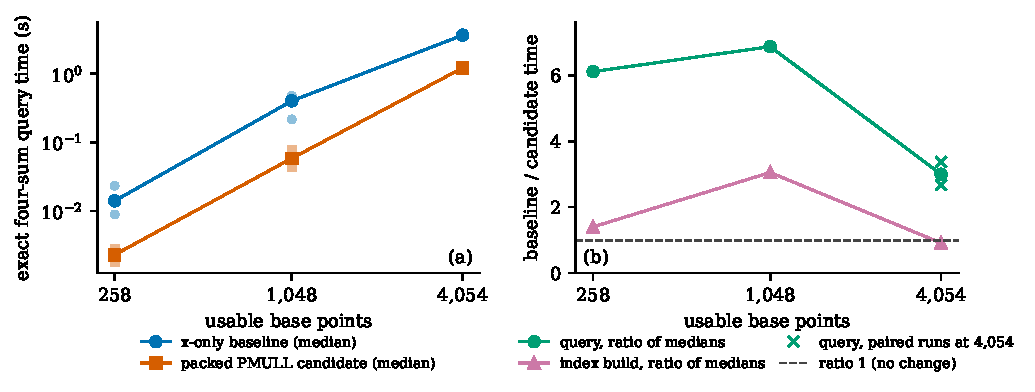
\includegraphics[width=\linewidth]{figures/fig-bin-pmull.pdf}
\caption[ARM64 PMULL arithmetic for the $n=83$ F6 query]{ARM64 PMULL arithmetic for the $n=83$ F6 x-only four-summand query
(field $z^{83}+z^{45}+z^2+z+1$, curve \texttt{icv1-f2m83-tm6151469093347-debefd74}).
(a)~Exact query time per run (light markers) and median (joined) for the
x-only baseline and the packed PMULL candidate, against the number of usable
base points: three runs per arm at 258 and 1{,}048 points, two at 4{,}054.
(b)~Baseline over candidate time: ratio of medians for the query and the index
build, and the two adjacent interleaved query pairs at 4{,}054 points
($2.674\times$, $3.372\times$). Medians and ratios are derived from the per-run
values in \texttt{figures/data-bin-pmull.json}. Every run returned the same
\texttt{no\_witness} outcome; a planted control recovered its witness with both
methods. One unisolated arm64 macOS host, no paired rho run: an exploratory
component diagnostic, not a controlled speed-up, with no end-to-end IC effect
measured (\art{research/f6_n83_pmull_xonly_20261005/RESULT.md}).}
\label{fig:bin-pmull}
\end{figure}

The algebraic gates of the same days ended open or negative. On the
registered K0 curve a standard dimension-18 subspace gives $261{,}447$
geometric points ($130{,}722$ sign-folded columns), and the direct
five-summand $\Sem3$ chain is exact on a planted control with 339 Boolean
variables and 332 cubic equations, smaller than the six-summand chain's 428
and 415, but its root-pruning gate fails
(\art{research/f6_n83_fivesum_d18_20261005/RESULT.md}). A recursive
carry-less (Karatsuba) circuit for the two dense $83\times83$ products of the
middle links passed its encoding gate and the solver timed out
(\art{research/f6_n83_karatsuba_sat_20261005/RESULT.md}). No natural relation
came from F6 at $n=83$.

\paragraph{October 24: every descent engine had been wrong.} A summand sweep
with every engine on the pinned $n=83$ fixture (53-bit subgroup) found the
same truncation one level lower: \texttt{FieldStructure} truncated the field
table to one 64-bit word, and every Weil-descent engine (matrix F4, matrix
F5, inherited F4, F6-IC, the F6-IC pair index, crossbred, SAT descent in
three encodings and MQ-FES) returned ``proved \textsc{unsat}'' on
\emph{planted} $n=83$ relations (\art{research/n83_msweep_20261024/README.md}).
The descent builders now refuse such a field, a regression test pins it, and
every earlier $n=83$ engine refutation is void
(Table~\ref{tab:corr-xref}). On the corrected build:
\begin{itemize}
\item chained-$\Sem3$ full-width SAT is the only decomposer that runs at
  every $m$, and within its 180-second cap it decides only $m=2$: 17.3\,s per
  public query (4 of 4 refuted) and 2 of 2 planted witnesses recovered. Its
  derived projection is $2^{75.9}$\,s, $2^{75.3}\times$ rho;
\item the $m=4$ root finder solves the complete DLP at $K=1107$ in
  $188.5$ and $175.2$\,s against a strong-rho mean of $1.509$\,s,
  $116$--$125\times$ from rho;
\item on the degree-61 companion field at $m=2$, native-XOR SAT is the
  fastest decider at $D\ge12$ (0.79--2.41\,ms per query) and inherited F4
  the fastest Gr\"obner engine (6.2--33.4\,ms); $m\ge3$ is refused by the
  64-variable descent mask.
\end{itemize}

\paragraph{October 31 to November 1: chained SAT becomes a lookup.} Six
frozen-protocol follow-ups extended chained SAT to $m=9$ by putting
root-finder tables and a $|B|^d$ meet-in-the-middle lookup in front of it;
by the last step no decided target makes a SAT call
(Table~\ref{tab:n83l-sat}, \S\ref{sec:n83l-sat}). The engine became a
generic meet in the middle. These are decomposition-stage measurements with
no complete DLP and no matched-rho comparison, and the registry counts the
lookup outside its 79+24 (\S\ref{sec:em-inventory}).

\section{What the Boolean engines settle}\label{sec:bo-summary}

Across the four families the record is consistent.
\begin{itemize}
\item Every accepted engine change is a component speed-up of the same
  search: identical verdicts, identical trees or traces, a faster
  representation. The largest complete-call factor is the F5 support cut
  ($3.0\times$); most preregistered candidates failed a $1.05$ gate.
\item Priced inside a whole solve, the algebraic engines are $22$--$33\times$
  (inherited F4, $n=13$) to $10^2$--$10^4\times$ the frozen strong rho, and the
  gap grows with $m$ (\S\ref{sec:bo-inherited}). Against the v2 reference of
  \S\ref{sec:em-accounting} these distances are roughly $3$--$5\times$ larger
  at $n=13$--19.
\item Where an engine became much faster on index-calculus systems (F6-IC
  with the few-candidate closure, chained SAT with tables and lookups), it did
  so by becoming the meet-in-the-middle oracle, whose relation cost is
  bounded below by \S\ref{sec:gf-collision}.
\item Two field-width defects (4 and 24 October) made engines report
  refutations that were not proofs; the second was found by planted
  relations and voided every earlier $n=83$ engine refutation.
\end{itemize}
The open engine question the atlas leaves is the one the closure
measurements of Chapter~\ref{ch:instruments} address: a descended cell
where the pair table is infeasible and the algebraic degree stays bounded.
\chapter{Prime and extension-field Gr\"obner engines}\label{ch:fpengines}

Over $\FF_p$ and $\FF_{p^k}$ the decomposition system is not Boolean, and
the engine is an $\FF_p$ F4: \texttt{f4\_fp} for generic systems,
\texttt{f4\_fp\_tower} with a Faug\`ere--Lachartre block for the
Kummer-tower systems of \S\ref{sec:pkm}, a signature variant, and for $k=4$
the weighted Macaulay solves of Chapter~\ref{ch:extension}.
Chapter~\ref{sec:groebner} lists \texttt{f4\_fp}'s headline ratios
($29.8$--$54.1\times$ over its predecessor, msolve parity $0.96$--$1.22$).
This chapter gives the arithmetic rounds behind them, the external
references, the one study that priced a faster \texttt{f4\_fp} end to end,
the Kummer-tower engine at large primes, the chain-solve levers on the GLS
$\FF_{p^4}$ line, and F4 trace replay. As in Chapter~\ref{ch:boolean}, an
engine gain is a component result until a whole solve is priced against
rho, and on every line in this chapter rho stays ahead.

\section{Arithmetic of the $\FF_p$ F4}\label{sec:fe-arith}

The $\FF_p$ rounds used the gate of \S\ref{sec:bo-gate}: one binary, paired
A/B blocks with an A/A floor, exact basis and solution fingerprints, step
counts and matrix shapes on 13 cases, holdout seeds, and a preregistered
promotion threshold on the complete F4 call of \texttt{quad\_n8\_p65521}.
\begin{itemize}
\item \emph{Narrow 32-bit rows} (\art{research/fp_f4_narrow_20260926/RESULT.md}).
  The branch-free 32-bit path read $1.113$ $[1.111,1.121]$ and missed its
  $1.2\times$ gate. Deferring reductions across each row's pivots (mode 2)
  read $1.641$ $[1.631,1.649]$ on one thread and $1.580$ on four, with
  $2.101\times$ on the overdetermined $n=12$ case; a default-on confirmation
  ($1.640$ one thread, $1.480$ four threads) made mode~2 the default for
  $p\le65{,}536$.
\item \emph{Lazy vector accumulation.} An AVX2 lazy accumulator read
  $1.059\times$ $[1.055,1.062]$ over the deferred default and $1.756\times$
  over the original 64-bit arithmetic, below its $1.15\times$ promotion gate
  and with two smaller-case regressions
  (\art{research/fp_f4_lazy_avx2_20260928/RESULT.md}); the AVX-512 version
  read $1.047\times$ and $1.513\times$ on an Intel host and stays
  hardware-gated and opt-in
  (\art{research/fp_f4_lazy_avx512_20260928/RESULT.md}). The two hosts
  differ, so the two results are not multiplied.
\item \emph{Where the time went by 29 October.} On a shared 4-vCPU host,
  one thread, \texttt{f4\_fp} was level with msolve~0.6.5 on
  \texttt{quad\_n8} ($47.8$ against $47.4$\,ms, msolve including start-up)
  and faster on seven other systems; 44\% of instructions on
  \texttt{quad\_n9} were in one multiply-accumulate kernel, and at four
  threads the reduce phase was still 66--84\% of the run, with one
  in-block dependency loop running on a single thread
  (\art{research/f4_f5_followups_20261029/README.md}). The two candidates
  aimed at those findings were exact and did not save time
  (\S\ref{sec:bo-gate}).
\end{itemize}
An independent campaign in \texttt{cryptanalysis} reported symbolic
preprocessing $2.34\times$ ($fb=3$) and $1.99\times$ ($fb=4$) faster on Semaev
systems and Boolean F5B-family bases $1.36$--$1.49\times$ faster, on a shared
host under load averages above 40; its README calls this local progress,
not a speed record (\art{cryptanalysis:experiments/groebner-perf-20260924/README.md}).

\section{External references}\label{sec:fe-external}

Two external comparisons frame what an in-house engine ratio means.
\begin{itemize}
\item \emph{msolve.} A day before the parity result of
  Table~\ref{tab:prog_groebner-engineering}, msolve was $12$--$24\times$
  faster than \texttt{f4\_fp} on square systems; after the rewrite the
  ratio is $0.96$--$1.22$ single-threaded, and the follow-up above found
  parity or better on eight small and medium systems. The parity is on
  generic square systems, not on the decomposition systems.
\item \emph{Magma.} A protocol registered on 13 October, before any Magma
  output, exports the exact systems behind the repository's Gr\"obner claims:
  26 Kummer-tower systems at $p=2{,}013{,}265{,}921$, five $k=4$ systems and
  eight Boolean root systems of the $n=17$ search, every one a unit ideal in
  the repository's runs (\art{research/magma_f4_comparison_20261013/PROTOCOL.md}).
  The directory holds the export bundles and the repository's own timings;
  no Magma output is committed, so the comparison has not been made.
\end{itemize}
The desk review of 24 October (\S\ref{sec:corr-engine}) puts these in
proportion: on the PKM systems the in-house F4 needed $10^3$--$10^7$ more
operations than a brute grid on the same base, so ratios of a root finder or
a table to that F4 (such as those of \S\ref{sec:rootfinding}) say nothing
about published Gr\"obner solvers. Solving \emph{degrees} measured with
msolve are unaffected.

\section{A faster \texttt{f4\_fp}, priced end to end}\label{sec:fe-e2e}

One study measured what the \texttt{f4\_fp} rewrite (PR~\#1717) did to a
complete index calculus in which every decomposition is one \texttt{f4\_fp}
solve: Nagao decompositions on a genus-2 cover of $E(\FF_{p^6})$, the same
seeds and relations in both arms, every logarithm correct
(\art{research/f4_fp_ic_effect_20261018/README.md}). Per decomposition test
F4 used $7.7\times$ fewer multiplications and the cover's counted cost
$5.0\times$ less (at $p=53$, 101, 251). End to end:

\smallskip
\begin{center}\small
\begin{tabular}{@{}lrrr@{}}
\toprule
$p$, seed & $S$ before/after & $S$/rho before & $S$/rho after \\
\midrule
53, 1 & $5.05$ & $4{,}297$ & $850$ \\
53, 2 & $4.99$ & $1{,}843$ & $370$ \\
101, 1 & $5.06$ & $981$ & $194$ \\
101, 2 & $5.08$ & $1{,}897$ & $373$ \\
\bottomrule
\end{tabular}
\end{center}
\smallskip

\noindent This is the one case in the programme where an $\FF_p$ engine gain
passed through to the whole solve almost unchanged ($5.0\times$ of a
per-test $5.0\times$), because the cover's decomposition is the solve. The
$S$/rho columns are a lower-bound comparison: neither arm emits its unpriced
native work, so no band applies. The distance after the change is
$194$--$850\times$; the cover itself is the subject of \S\ref{sec:transfer}.

\section{Kummer-tower engines at large primes}\label{sec:fe-pkm}

The tower F4 engine held coefficients in \texttt{u32}, which left the
Kummer tower at 2-adic valuations $v_2(p-1)\ge40$ unmeasured. A generic-field
engine (\art{research/f4_generic_field_20261015/README.md}; protocol frozen
before any measured cell; shared host, L0) ports the same algorithm to any
prime field.
\begin{itemize}
\item At \texttt{Fp32} it reproduces \texttt{f4\_fp\_tower} field for field:
  182 rows of every round-8 series with $N\le18$, zero differences in degree,
  width, steps, multiply-adds and every counter; and it is not slower
  (paired $u32$/generic $1.091$ and $1.058$).
\item Above $2^{31}$ it is $2.18\times$ ($m=2$, $N=16$) and $2.24\times$
  ($m=3$, $N=12$) faster than the \texttt{u32} engine with eager Barrett
  reduction, and at 45 bits an AVX-512 IFMA backend is $2.57\times$ the
  64-bit one; five of five preregistered claims pass.
\item The solving degree is independent of $v_2$ and of the prime's size in
  every valued cell: Kummer towers at $v_2=40,48,56$ and at the P-224
  prime, and the Dickson torus at P-192 and P-256, give the 31--32-bit
  degree, width and step count. At $m=2$, $N=18$ the multiply-add count is
  $45{,}952{,}850{,}022$ at 45, 52, 61 and 224 bits.
\end{itemize}
The last point is the engine-side complement of \S\ref{sec:pkm}: the
tower's degree is a property of the system shape, and the prime only
changes the cost of a multiplication. In ecbench the four PKM tower engines
(F4, F5, F6 and geometric enumeration) all run and read $4.62$--$5.03\times$
negation rho on the current binary (\S\ref{sec:em-frontier}); the
presentations that change the system shape are in \S\ref{sec:pa-pkm}.

\section{The chain-solve levers on the GLS $\FF_{p^4}$ line}\label{sec:fe-chain}

Chapter~\ref{ch:extension} gives the $k=4$ engineering ladder to 15 October.
In parallel a second line of work moved the same problem onto a
Klein-four ($V_4$) invariant line on GLS curves over $\FF_{p^4}$ and ran
pre-registered experiments E17--E42 (the $V_4$ line from E22, 18 October), each recorded in the research note
\art{research/notes/index-calculus/RESEARCH_GLV_INVARIANT_FACTOR_BASES.md}
\S9 with its own report directory. On this line the decomposition solve is
$97.7$--$98.5\%$ of $S$ and the linear algebra at most $0.006\%$
(E32, \S9.36), so the solve's Macaulay matrix ($393\times448$ at degree 11,
$176{,}064$ dense cells per call) is the whole cost. The levers below act on
that matrix. Each is priced in the line's own unit,
\[
  S(g)=\text{counted }\FF_p\text{ multiplications}
  + 97g\,(\text{Macaulay entries}+\text{selection work}),\qquad g\in\{0,0.1,1\},
\]
which is the band of \S\ref{sec:band} with a native operation priced at
$97g$ multiplications, and each is ranked against its predecessor only where
the order holds at all three weights on every row.

\paragraph{The baseline: chain solve and handover ladder.} E31 replaced the
existing solve (E25's) by its $P_2$-chain solve with identical decompositions
on every call: solver~A cut the multiplications per call $2.62$--$2.69\times$
and solver~B (sparsest pivots) $4.99$--$5.32\times$. End to end, $S_{E25}/S_A$
is $2.50$--$2.56\times$ at 0~GAE, $1.39$--$1.43\times$ at 0.1 and
$1.034$--$1.053\times$ at 1, so A is ranked ahead across the band. B is ahead of E25 at every weight
as E31 counted it, but with its selection pass priced (E33, below) it falls
behind E25 at 1~GAE and is unresolved
(\art{research/e31_chain_solve_20261024/}; validated, \texttt{VAL-20261024-24ef8b},
\art{benchmarks/20261024-e31-chain-solve/VALIDATION.json}; validation-gate
pass, no pcc claim, so an unverified assertion under the 4 November rule). E32 then measured
the distance over eleven sizes, $\log_2n=22.6$--$42.4$, 33 paired curves:
rho is ahead on every curve at every weight, the best curve is $1{,}143\times$
from rho at 0~GAE, the fitted slope of the distance is $-0.243$
$[-0.279,-0.205]$ in $\log_2n$ (Gaudry's $-1/4$), and the extrapolated
crossover order is $2^{85.5}$ $[2^{79.2},2^{94.3}]$ at 0~GAE, $2^{91.2}$ at 0.1
and $2^{97.6}$ at 1 (\art{research/e32_handover_ladder_20261031/}; validated,
independent replay of 66 of 66 runs). The crossover is an extrapolation 37--66
bits past the top size, not a measured crossing.

\paragraph{The levers.} Table~\ref{tab:fe-levers} lists the solver and
storage levers that followed, each against the ranked solver~A.

\begin{table}[t]
\centering\small
\begin{tabularx}{\linewidth}{@{}l>{\raggedright}p{0.25\linewidth}>{\raggedright}p{0.2\linewidth}>{\raggedright}X>{\raggedright\arraybackslash}p{0.13\linewidth}@{}}
\toprule
& Lever & $S_A/S_X$ at $0$ / $0.1$ / $1$ GAE & Rank against A & Standing \\
\midrule
E33 & B with its selection counted ($1.05\cdot10^6$ ops/call) & $1.82$--$1.86$ / $0.193$--$0.197$ / $0.149$--$0.152$ & unresolved (ahead at 0 only) & validated \\
& B$''$ (Markowitz estimate, $\approx1.27\cdot10^4$ ops) & $1.538$--$1.558$ / $1.046$--$1.048$ / $0.9465$--$0.9480$ & unresolved (behind at 1) & validated \\
E35 & T: B's pivots learned per curve, replayed & $1.093$--$1.252$ / $1.020$--$1.055$ / $0.998$--$1.003$ & unresolved (6 of 20 rows behind at 1) & producer \\
E39 & F: first-arrival pivots, no selection work & $1.457$--$1.537$ / $1.094$--$1.106$ / $1.0115$--$1.0130$ & \textbf{ahead} on 32 of 32 rows & validated \\
& S: static order & $1.402$--$1.449$ / $1.083$--$1.091$ / $1.0077$--$1.0086$ & \textbf{ahead} & validated \\
& H: F with static fallback & $1.497$--$1.542$ / $1.096$--$1.103$ / $1.0076$--$1.0083$ & \textbf{ahead} & validated \\
E40 & V: rows stored from their lead & $1.0000$ / $1.2518$--$1.2618$ / $1.3629$--$1.3807$ & equal at 0, ahead at 0.1, 1 & validated \\
E42b & W: V's tails reserved to the fill (vs V) & $1.0000$ / $1.022$--$1.023$ / $1.032$--$1.034$ & equal at 0, ahead at 0.1, 1 & producer \\
\bottomrule
\end{tabularx}
\caption[]{Chain-solve levers on the GLS/$V_4$ line, end to end, ranges over
the paired rows (20 rows for E33 and E35, 32 for E39--E42b); above 1 the
lever is cheaper. E42b is against V, not A. Rho is ahead of every row at
every weight. ``Validated'': the study directory or its \texttt{benchmarks/}
copy carries a \texttt{VALIDATION.json} with a passing independent validator
report. Sources: \art{research/e33_solver_b_pivot_count_20261031/REPORT.typ},
\art{research/e35_chain_trace_20261102/REPORT.typ},
the research note \S9.49 and \art{research/e39_pivot_rules_confirm3_20261102/},
\art{research/e40_macaulay_entries_20261102/REPORT.typ},
\art{research/e42_macaulay_tails_20261103/REPORT.typ}.}
\label{tab:fe-levers}
\end{table}

Read across the table, the band does the ranking work it was built for.
\begin{itemize}
\item \emph{A gain that exists only at 0~GAE.} Solver~B multiplies
  $1.82$--$1.86\times$ less than A, but its pivot selection reads the matrix
  about six times per call. Counted, B and its cheaper twin B$'$ fall behind
  A from 0.1~GAE, and the Markowitz estimate B$''$ falls behind at 1~GAE,
  where its $1.2\cdot10^6$ priced multiplications of selection exceed its
  $2.3\cdot10^5$ saving (E33). The validator report states that E33 claims no
  improvement across the band.
\item \emph{A pivot order that is not a property of the curve.} If B's
  choices were fixed per curve they could be learned once and replayed,
  as in Joux--Vitse F4 trace reuse~\cite{jouxvitse2012}. E35 found that no
  call's pivot sequence equals its curve's trace and that 997--1{,}000 of
  1{,}000 sequences per curve are distinct; in contested columns B's row
  agrees with the trace in $69.8$--$88.4\%$ of cases, and another curve's
  trace agrees as well. The replay keeps $18.8$--$36.8\%$ of B's saving and
  is break-even with A at 1~GAE.
\item \emph{A gain at every weight.} Taking pivots in arrival order (F)
  removes the selection pass entirely and still cuts A's per-call cost
  $1.47$--$1.55\times$. E36 and E37 showed F, S and H ahead of A at every
  weight, but each time a pre-registered kill criterion fired on a
  control's positive check, so neither ranked them; E38's kill fired at its
  pilot. E39, the third confirmation, used a control that alters a read
  pivot row after its last use, no kill fired, and F, S and H are ranked
  ahead of A and E25 at 0, 0.1 and 1~GAE on all 32 rows, under three
  alternative pricings as well (validated, \texttt{VAL-20261102-E39};
  \art{benchmarks/20261102-e39-pivot-rules/}). At 1~GAE the margin is
  $0.8$--$1.3\%$.
\item \emph{Gains that exist only at positive weights.} Storing each row
  from its lead (V) leaves the arithmetic untouched: $41.6\%$ of the
  $176{,}064$ cells lie left of each row's lead and are never read by the
  echelon, so V equals A at 0~GAE and is ahead only where a stored cell has
  a price (E40; validated, \texttt{VAL-20261102-E40}). W reserves each row
  only to the block after its build end and is ahead of V by $2.2$--$2.3\%$
  at 0.1 and $3.2$--$3.4\%$ at 1~GAE (E42b). The report classifies it as a
  data-structure constant; its size is set by the per-cell price.
\item \emph{A kill by the study's own control.} E42 registered a range of
  $[900,960]$ re-allocations per call for its growth control, derived from
  the wrong counter; G0 made $245.6$, the kill fired, and W stayed
  unranked. E42b re-registered the question, with the range derived from
  W's own overflow rule ($[200,300]$; measured $246.3$), before any ranking
  data existed (Table~\ref{tab:corr-engine}). E42b has no validator report.
\end{itemize}

\paragraph{Distance.} None of these levers is an end-to-end change of the
distance in kind. The best rows of the table sit at $S_X/\text{rho}$ of
$5.15\cdot10^3$ (H, 0~GAE) to about $6\cdot10^3$ (V and W, 0~GAE), rising to
$5.97\cdot10^4$--$9.4\cdot10^4$ at 1~GAE; the worst rows reach
$2.3\cdot10^5$ at 0~GAE and $7.0\cdot10^6$ at 1~GAE. Measured against the success criterion E31,
E39 and E40 are validation-gate improvements of the index-calculus baseline
(no pcc claim exists for any of them, so each is an unverified assertion
under the 4 November rule; E39
across the whole band, E40 at positive weights), each a constant on one
stage; measured against rho they leave the gap where E32's ladder put it,
closing as $n^{-1/4}$ with an extrapolated crossover near $2^{85}$--$2^{98}$.

\section{Trace replay as a component speed-up}\label{sec:fe-trace}

Joux and Vitse's observation~\cite{jouxvitse2012} is that the F4 runs of one
decomposition family share their sequence of useful rows, so one run can be
recorded and later runs replayed. The programme tried it on four objects.
\begin{itemize}
\item \emph{Binary $\Sem3$ chain.} Learn/apply trace reuse gave
  $1.4$--$2.3\times$ in \texttt{cryptanalysis}, and the whole Boolean-engine
  lead is closed as dominated by the pair table
  (\S\ref{sec:bo-inherited}).
\item \emph{The $k=4$ weighted solve (E21, 18 October).} Over 400 targets at
  $p=53$ and 101 the replay agreed on every decomposition set but fell back
  on $13$--$23.5\%$ of targets, because which rows reduce to zero is not
  stable across targets of one curve; the total cost with fallbacks was
  $0.95$--$0.98\times$ of the full solve, a net loss (research note \S9.11).
\item \emph{The chain solve's pivots (E35).} No per-curve order exists
  (\S\ref{sec:fe-chain}).
\item \emph{The PKM--Semaev oracle on Curve25519 miniatures (2 November).}
  \texttt{f4\_fp\_tower} gained \texttt{record\_trace} and \texttt{replay}: a
  recording run keeps, per F4 step, the S-rows whose residue gave a new
  pivot and the reducers they reached; a replay forms only those rows and
  stops at the first step whose leads differ. Only a refutation is a result
  of a replay (every row lies in the ideal, so reaching 1 is sound whatever
  the trace was learned on), and a non-refuting replay falls back to plain
  F4, charged (\art{research/curve25519_f4_trace_20261102/README.md}).
\end{itemize}
The fourth object is the one where the idea works, and its numbers show the
size of a trace-replay gain (Table~\ref{tab:fe-trace}).

\begin{table}[t]
\centering\small
\begin{tabular}{@{}rrrrrrr@{}}
\toprule
$t$ & $G$ & plain/target & trace/target & trace/plain & break-even $n^*$ & fallbacks/replays \\
\midrule
6 & 0 & $5.55\cdot10^7$ & $2.25\cdot10^7$ & $0.41$ & $1.68$ & 0/100 \\
6 & 4 & $7.10\cdot10^5$ & $3.23\cdot10^5$ & $0.45$ & $1.83$ & 0/1{,}600 \\
7 & 0 & $7.46\cdot10^8$ & $2.35\cdot10^8$ & $0.32$ & $1.46$ & 1/100 \\
7 & 4 & $9.70\cdot10^6$ & $4.13\cdot10^6$ & $0.43$ & $1.74$ & 0/1{,}600 \\
8 & 0 & $6.98\cdot10^9$ & $2.32\cdot10^9$ & $0.33$ & $1.50$ & 4/100 \\
8 & 4 & $8.64\cdot10^7$ & $3.85\cdot10^7$ & $0.45$ & $1.86$ & 6/1{,}554 \\
\bottomrule
\end{tabular}
\caption[]{F4 trace replay in the PKM--Semaev oracle, Curve25519 $k=20$
miniature, $m=2$, 100 targets per cell, in F4 elimination multiply-adds per
target (learning excluded; $n^*$ is the number of targets after which
learning has paid back). Selected cells of nine. Source:
\art{research/curve25519_f4_trace_20261102/README.md}.}
\label{tab:fe-trace}
\end{table}

\noindent Replay costs $0.29$--$0.45$ of plain F4, learning costs one plain
run per branch system, and it pays back after about two targets. The
preregistered prediction that replay would cost at most $0.25$ of plain at
$G=0$ failed ($0.29$--$0.41$). The gain is a component gain in the oracle's
own unit; the README states that nothing is claimed for wall time, other
sizes or against rho. Priced end to end, a $t=4$, $G=3$ arm with trace
replay costs $0.2837$ $[0.2413,0.3335]$ of the previous Curve25519 winner at
$w=0.1$ and $1.567\times$ more at $w=0$, so the order flips inside the band,
and it is still $27.9$, $1.83\cdot10^4$ and $1.13\cdot10^5\times$ rho at
$w=0,0.1,1$ (\S\ref{sec:c25519};
\art{research/curve25519_t4_candidate_ecbench_20261104/validator-report.json},
status \texttt{pass\_with\_errata}).

Across the four objects the pattern is the one E21 and E35 state: trace
replay pays where the useful-row structure is a property of the system
shape (the PKM tower, the binary chain) and fails where it depends on the
target (the weighted $k=4$ solve, sparsest-pivot choices). Where it pays it
is a constant between about $1.4\times$ and $3.4\times$ on the oracle, which the
relation phase's yield then divides.
\chapter{Degree instruments, linear algebra and planners}\label{ch:instruments}

The engines of Chapters~\ref{ch:boolean} and~\ref{ch:fpengines} solve; the
tools of this chapter measure, finish or choose. A degree instrument
measures the degree at which a system refutes, which sets the exponent of an
algebraic oracle long before any end-to-end run is affordable. The linear
algebra finishes the index calculus once relations are collected. Planners
and autolabs choose factor bases, oracles and parameters. A GPU line and a
hashed-ECDL engine measure how far explicit relations reach in practice.
Each kind of tool has its own way of being wrong, and the record below is
mostly about those.

\section{Closure and guess instruments}\label{sec:in-closure}

\S\ref{sec:binary} reports the closure-degree measurements to 24 October: a
MutantXL-style closure refutes the chained $m=3$ descent systems at degree
3--4 where XL needs 5--7, stays at degree 4 up to $\ell=6$, and rises past 4
at $(m,\ell)=(3,7)$; guessing one or two variables restores degree 4 there at
$1/116$--$1/260$ of the projected degree-5 cost. The $\ell=8$ guessed-variable
series that followed (four guesses suffice, three do not for one set, the
$(22,7)$ null, the invariant guesses, and what they price for ECC2K-130) is
reported in \S\ref{sec:bd-guess} and Table~\ref{tab:bd-guess}. This section
describes the instrument and the control lesson behind every row of that
table.

\paragraph{The instrument.} \texttt{dreg\_closure} builds the Macaulay
closure of one draw's system degree by degree, records the closure and XL
ranks, the columns and the word operations at each degree, and scores a draw
as refuting at the first degree whose closure contains the constant.
\texttt{dreg\_score} scores the records against a preregistration. Every
study of Table~\ref{tab:bd-guess} fixes a cell, draws unsatisfiable and satisfiable systems from a
seed, and runs three controls: an identity control that reproduces an
earlier committed record field for field, a positive control (a guess set
known to refute), and a negative or null control that must \emph{not}
refute.

\paragraph{A null control that failed.} The specialisation study of 17
October is the counter-example that justifies the controls. Fixing one
variable brought most $\ell=7$ draws back to degree 4, but the null control
refuted on 6 of 8 draws where at least 7 of 8 had to fail, so the registered
verdict was ``uninformative''
(\art{research/dreg_closure_specialise_20261017/RESULTS.md}). Without the
null, ``one fixed variable restores degree 4'' would have read as a
structural finding.

\section{The linearization-excess rule}\label{sec:in-excess}

For two summands a structural number, the linearization excess
$e=n-\dim V-\dim V^{(2)}$ of a subspace factor base $V$, predicts the
closure solving degree before any solve, $D=2+[e<-3.5]+[e<-8.5]$ over 656
bases at mean absolute error $0.06$; the rule, the progression bases it
singles out and the $m=3$ formulation point are stated in full in
\S\ref{sec:bt-fbselect} (\art{cryptanalysis:experiments/pdp-degree-heuristics/README.md}).
None of it is an index-calculus result: every row is a decomposition-stage
profile on small fields. The atlas lead that would transfer it (rank
candidate bases of equal size by $e$ inside the $m=3,4$ closure cells of
\S\ref{sec:bd-guess} and measure degree and charged cost with a random
control) is \emph{open, unexamined}
(\art{crypto-autoresearcher:knowledge/leads/ecdlp/ic-engine/LEAD-ICE-linearization-excess-fb-prior.yaml}).

\section{Presentations as an instrument}\label{sec:in-presentation}

The same decomposition can be written as different systems, and a system's
solving degree, not the decomposition, is what an engine pays for. Two
studies of late October measured that freedom directly.

\paragraph{Tree-glued encodings.} A tree-glued, cherry-symmetric encoding
$T$ of the prime-field point decomposition (each summand pair encoded by its
symmetric functions with a degree-2 remainder tower, pairs glued by
$\Sem3$, every input of degree at most 4 for every arity) was compared with
the plain chain $C$ and the full symmetric arm $F$ under msolve~0.6.5 on
identical Kummer-base targets (\art{research/ic_tree_gluing_20261103/README.md};
stage diagnostic, no $S$, contended timings).
\begin{itemize}
\item Against $C$, $T$ is better in every completed cell: at $m=2$ its
  degree stays 4 for $t=3$--7 while $C$ rises to 5 at $t=6,7$, with matrices
  $1.8$--$3.6\times$ narrower; at $m=3$, $t=5$ it finishes at $D=6$ while $C$
  is cut off in degree 7; at $m=4$, $t=4$ it finishes at $D=7$ in 697\,s.
\item Against $F$ it loses on cost at $m\le4$: at $m=3$, $F$ reaches $D=5$
  against 6 at $t=4$, and at $m=4$ the recorded $F$ row ($D=8$, from a different
  engine) was $59\times$ faster.
\end{itemize}
Six further rounds (\art{research/ic_tree_gluing_20261103/STATUS.md}, all
\texttt{[pcc:unverified]}, four round-5 statements under claim records)
measured a coupling excess $E=D_T-4$ of 0, 2, 3 at $m=2,3,4$ and at least 5
at $m=5$ (memory exhausted at 14.5\,GiB), about $+1.5$ per summand and $+0.5$
per tower level; no encoding, symmetry or branching tried moved either slope.
The line is recorded as closed at cryptographic sizes under the measured laws
and open asymptotically on whether $E$ grows by at most one per summand, a
question its deciding cells cannot answer under 15\,GB.

\paragraph{Contraction order on $\FF_{p^3}$.} The atlas lead on planning the
contraction order of a Semaev network
(\art{crypto-autoresearcher:knowledge/leads/ecdlp/ic-engine/LEAD-ICE-gag-contraction-planner.yaml})
was tested at $n=m=3$ over $\FF_{p^3}$, $p\in\{1009,4099,32749\}$, 30 planted
instances, under a frozen \texttt{experiment.protocol/v1}
(\art{crypto-autoresearcher:research/gag_presentation_matched_20261031/README.md}).
All arms returned identical verified relations. The monolithic $\Sem4$
presentation used $0.110\times$ the chained presentation's F4 matrix cells at
every prime (verdict \emph{supported within scope}, descriptive); the tree
presentation used $1.095\times$ and is inconclusive, because one charged
retry set the $p=1009$ A/A floor. An independent \texttt{review-run}
recommends replication, and a filed correction fixes two statements of the
report (one instance, not three, has two decompositions) without changing a
verdict. Matrix cells are a stage unit; the study prices no pipeline and
makes no wall-time or rho statement.

\paragraph{Reading.} Both studies say the same thing in different units: a
presentation can lower the solving degree or the matrix size of a fixed
decomposition by a constant factor, and in the tree line the slope in $m$ and
$t$ stays. Chapter~\ref{ch:falldegree} gives the degree theory these
measurements test.

\section{The degree-of-regularity forecast}\label{sec:in-forecast}

A factor-base sweep decides one decomposition system per probe target and
learns the cell's degree of regularity for certain only once the relation
phase has run. The forecast \texttt{dreg\_forecast/v1}
(\art{src/cryptanalysis/dreg_forecast.rs}) estimates it from the solves so
far.
\begin{itemize}
\item A decided solve observes the solving degree $D$; an exhausted solve
  observes only $D>c$ for the highest completed degree $c$, a
  right-censored observation. The Kaplan--Meier estimator of $P(D>d)$ with
  Greenwood's standard error gives the predicted degree (the median) and a
  95\% band; a weak prior centred half on the semi-regular degree keeps it
  defined before the first decided solve.
\item The semi-regular degree of the system shape is the yardstick: a cell
  whose band lies below it is extracting structure.
\item The cost side projects the remaining relation phase from the
  observed per-degree work and yield, charges the relation matrix from its
  own row operations, and reports the rho floor over that work at 1, 10 and
  100 multiplications per group addition; advice is given after four real
  solves and ranks only where the order holds across that band.
\end{itemize}
The \texttt{dreg-triage} skill wraps it as a loop (plan, run, triage, refine),
and both the module and the skill state its limits: it is advisory, never
stops or shortens a candidate, leaves \texttt{certified\_degree\_of\_regularity}
null, and is a stage diagnostic, never a complete-DLP result
(\art{.agents/skills/dreg-triage/SKILL.md}). Its estimator is the same
censoring logic that statistics version~2 applies to engine costs
(\S\ref{sec:em-stats}), applied to degrees.

\section{Linear algebra}\label{sec:in-la}

The model of Chapter~\ref{ch:model} lists the linear-algebra levers
(structured Gaussian elimination, a CADO-style filter, Wiedemann's
algorithm~\cite{wiedemann1986} and its block form~\cite{coppersmith1994}, a
first-dependency stop). The measurements say that those levers are
available and are almost never the bottleneck.

\paragraph{Against CADO-NFS.} On synthetic $m=3$ relation systems over a
62-bit prime, in one session on a shared host
(\art{research/la_engines_20261014/README.md}; protocol and five amendments,
each before its data):
\begin{itemize}
\item the linear algebra is $0.11$--$1.9\%$ of 27 real \texttt{ic logs}
  precomputes, and the largest real index-calculus matrix in the repository
  (N73, 600 columns) took 5.1\,h to collect and milliseconds to solve;
\item the repository's block Wiedemann beats CADO-NFS \texttt{bwc} on the
  identical matrix at every size measured, $1.86\times$ at $131{,}072$ columns;
\item CADO-NFS's filter left a $5$--$8\times$ smaller matrix than the
  repository's; the port of that filter runs $86.57\to8.35$\,s at
  $D=262{,}144$ ($10.40\times$ $[9.99,11.06]$) and is $1.93\times$
  $[1.74,1.96]$ faster than CADO-NFS's own pipeline on the same matrices
  ($7.83$ against $14.73$\,s); below about 4{,}096 columns it is slower
  ($0.40\times$ at 1{,}024, both in milliseconds);
\item ecbench's default \texttt{IncrementalGauss} grows $6$--$9\times$ per
  doubling, $19.1$\,s at 8{,}192 columns.
\end{itemize}
These are component results in wall time at L0. The filter port is the
default of \texttt{ic logs} since.

\paragraph{Inside the pipeline: a null.} When the four sparse solvers were
made reachable from \texttt{ic.pipeline}, a paired study found that every one
costs \emph{more} end to end than the baseline: $1.206\times$ in total on an
$E(\FF_{29^4})$ $k=4$ ladder and $5.72\times$ falling to $1.030\times$ over
128--4{,}096 columns on a scaling curve
(\art{research/sparse_la_timing_20261018/README.md}). The cause is the
completion rule: the deferred solvers answer only at full column rank, while
\texttt{structured-gauss} and \texttt{incremental-gauss} stop as soon as the
target's column is pinned, so the full-rank arms collected $1.75\times$ and
$5.5$--$10.5\times$ more relations. A positive control with the same
full-rank rule and dense elimination reproduced the sparse arms' $S$. In
counted row operations the filtered solvers lose at every size; the
unfiltered Wiedemann and Lanczos count $10^3$--$10^4\times$ the row operations
of structured Gauss, growing as about columns$^{2.2}$.

\paragraph{Where it matters.} The exception is the GHS-weak plane quartic of
\S\ref{sec:transfer}, where double large primes shrink the factor base and
put linear algebra and relations both near $q^{1.0}$. There, structured
elimination (B1) was a stage gain of $0.81$--$0.91$ of the B0 cost up to
$q=65{,}479$ and a regression ($1.53$) at $q=262{,}111$, recorded as a trade
and not adopted; double large primes (B2) are the measured improvement,
$0.297$ $[0.295,0.299]$ of B0 at $q=262{,}111$
(\art{research/quartic_n4_la_20261021/README.md}). On the GLS $\FF_{p^4}$
line the linear algebra is at most $0.006\%$ of $S$ (\S\ref{sec:fe-chain}).
The relation phase, not the matrix, sets the cost on every line measured.

\section{Planners}\label{sec:in-planners}

\texttt{ic plan} chooses a factor base, oracle and parameters for a curve
from a cost model. Its validation on six curves is in \S\ref{sec:prime}.
Two later versions added weight rules (\texttt{ic-planner/2} a base of
$1.41N_0$ at $w=1$ on prime curves, \texttt{ic-planner/3} $0.71c_0$ on Koblitz
curves at $w\ge0.3$), and an exhaustive re-test of 26 October on 14 new
curves (3{,}328 records, 2{,}428 band verdicts restated in integers and
checked by Lean's \texttt{decide}) withdrew all three weight rules in
\texttt{ic-planner/4}: the prime rule failed its $w=0$ clause, the binary
rule failed at $w=1$, and the Koblitz rule was dearer at every weight
(\art{research/ic_planner_exhaustive_20261026/README.md};
\S\ref{sec:pg-engineering}, Table~\ref{tab:corr-xref}). The same re-test
found that the residual collector is cheaper than the plan across the band
from 36 bits, as a generic collision search, whose curve-free control costs
the same and whose exponent matches rho's (\S\ref{sec:pg-residual}).

\section{Autolab loops}\label{sec:in-autolab}

The autolab is the programme's loop for proposing and screening candidates
without letting the screen promote them. Its contract, used by the
tournament since September and by the native \texttt{ic\_autolab} loop since
4 November, has six steps: propose, build a portfolio, screen in sample,
select one challenger per size, confirm on fresh targets with the incumbent,
an A/A copy and the matched rho, and record the delta on a ratchet
(\art{.agents/skills/ic-autolab/SKILL.md}). The tool enforces what earlier
loops left to discipline: a round is frozen once, target seeds are disjoint
from every exposure, the in-sample screen never promotes, an improvement
needs the paired interval below 1 at $w=0$ and the band order at every
weight, and every arm joins the trial history so it is not proposed again.
Its first family, the Curve25519 miniatures, ran 35 rounds; the generic
incumbent settled at the collision floor derived in \S\ref{sec:c25519}, which
is the loop working as intended: the ratchet found the floor and could not
pass it. Earlier cycles (17--19 October) on the native GF($2^{83}$) norm
predicate are in \S\ref{sec:binary}. The loop's rows are development evidence
until the validation gate.

\section{Explicit relations on a GPU}\label{sec:in-gpu}

A separate line measured how far a complete prime-field recovery with
explicit relations reaches on one GPU: factor-base construction and generic
meet-in-the-middle relations on the device, elimination, scalar extraction
and certificate replay on the CPU, on public fixtures
(\art{research/explicit_relations_e2e_20261030/RESULTS.md}).
\begin{itemize}
\item Nine pinned versions recorded every launch, failures included. Version
  8 completed 12 of 12 recoveries through 60-bit fields on an RTX PRO 6000,
  with cold solves of $770.3$ and $845.2$\,s at 60 bits; version 9 recorded
  one 61-bit recovery and one memory refusal.
\item On an RTX 4090 a full-cache query kernel lowered the 63-bit cold
  recovery from $1{,}183.8$ and $1{,}185.8$\,s (baseline before and after) to
  $1{,}053.9$\,s, $11.05\%$ lower with a $0.164\%$ baseline repeat spread,
  certificates byte-identical (\art{research/explicit_relations_fullcache_20261101/RESULTS.md});
  linear algebra took $0.11$\,s of the $1{,}054$.
\item Block normalisation by a product tree uses 765 source-level field
  multiplications against 4{,}608 for dual scans, with no cold end-to-end
  gain established (\art{benchmarks/20261030-explicit-relations-gpu/}).
\end{itemize}
Every clock is L0 with \texttt{wall\_valid=false}; there is no matched rho
and no fastest-external-tool comparison, and the benchmark copy says it is
not an admitted result. The relations are generic meet-in-the-middle, so the
method is bounded by the collision floor of \S\ref{sec:gf-collision}; what
the line measures is engineering reach, not a distance.

\section{Hashed-ECDL engines}\label{sec:in-hashed}

The hashed factor base and the conditional tensor-contraction route are in
\S\ref{sec:pt-tensor}. Their CPU engine (\art{crates/hashed-ecdl-cpu/})
recorded two matched panels of 120 executions with byte-identical
certificates across arms; with persistent meet-in-the-middle tables and
batched inversions the complete known-answer solve fell from $45.99$ to
$3.90$\,ms ($p=65521$, $m=3$) and from $80.54$ to $4.12$\,ms ($m=4$), and from
$0.316$ to $0.283$\,ms at $p=211$ (\art{research/hashed_ecdl_cpu_20261030/README.md};
L0, one EKS VM). The larger-field ladder expired with zero executions. The
README states that these establish exact software behaviour on fixed
fixtures and no speed-up, matched-rho advantage or large-curve attack.

\section{Component speed-ups and end-to-end changes}\label{sec:in-summary}

Table~\ref{tab:in-summary} sorts the main results of this part by the three
labels of Chapter~\ref{ch:engmeasure}.

\begin{table}[t]
\centering\small
\begin{tabularx}{\linewidth}{@{}>{\raggedright}p{0.32\linewidth}>{\raggedright}X>{\raggedright\arraybackslash}p{0.22\linewidth}@{}}
\toprule
Result & Effect & Against matched rho \\
\midrule
\multicolumn{3}{@{}l}{\emph{Component speed-ups (identical outputs, stage unit)}} \\
F5 support cut 19 & complete call $3.0\times$ & not priced \\
Few-candidate F6-IC closure & CPU $2.67$--$10.29\times$ & reduces to MITM \\
Chained SAT with lookups, $n=83$ & $m$ up to 9 decided & no complete DLP \\
F4 trace replay (PKM--Semaev) & $0.29$--$0.45$ of plain F4 & $27.9$--$1.13\cdot10^5\times$ \\
CADO filter port & $10.40\times$ (filter) & LA $<2\%$ of solves \\
Generic-field tower F4 & $2.18$--$2.57\times$ & not priced \\
\addlinespace
\multicolumn{3}{@{}l}{\emph{End-to-end changes over an IC baseline}} \\
Faster \texttt{f4\_fp} in the cover pipeline & $S$ $4.99$--$5.08\times$ lower & $194$--$850\times$ (lower bound) \\
E31 chain solve (validated) & $S$ $1.03$--$2.56\times$ lower across band & $4.42\cdot10^3\times$ at best \\
E39 arrival-order pivots (validated) & ahead of A at every weight & $5.15\cdot10^3\times$ at best \\
E40 lead-stored rows (validated) & ahead of A at $w>0$ only & $6.00\cdot10^3\times$ at best \\
Generator-orbit base, Koblitz (validated) & $1.26$--$3.20\times$ & below rho only at $n=29$, one column (BSGS) \\
Harvest default, inherited F4 & $+9.6\%$ to $-4.1\%$ by size & $7$--$1{,}250\times$ (frozen strong) \\
\addlinespace
\multicolumn{3}{@{}l}{\emph{Accounting and instrument changes}} \\
Accounting v2 & references resized & gap larger \\
Statistics v2 & censored runs kept & engine ratios lower bounds \\
Allocator confound & wall time of small arms & counts identical \\
64-bit field truncation, $n=83$ & refutations voided & --- \\
\bottomrule
\end{tabularx}
\caption[]{The part's results by class. ``Validated'': a \texttt{VALIDATION.json}
with a passing validator report; every other row is producer-reported.
Sources in \S\S\ref{sec:em-accounting}--\ref{sec:in-gpu}.}
\label{tab:in-summary}
\end{table}

Three conclusions follow, each with its scope.
\begin{itemize}
\item \emph{The machinery works.} Engines reproduce each other and brute
  force, sessions replay to the last digit, defects are found by planted
  controls and pinned rather than hidden, and the band ranks levers whose
  sign depends on a price. That is a statement about the instrument, made
  by the instrument's own audits.
\item \emph{Engine gains are real and small against the gap.} The largest
  end-to-end engine change in this part is a factor of about 5 (the
  \texttt{f4\_fp} cover pipeline; producer-reported, lower-bound
  comparison). The largest validated ones are the generator-orbit base
  ($1.26$--$3.20\times$) and E31 ($2.50$--$2.56\times$ at 0~GAE,
  $1.03$--$1.05\times$ at 1~GAE), both validation-gate passes without a pcc
  claim. These stand against distances to rho of $10^2$ (Koblitz, binary, prime) to $10^3$--$10^6$
  ($\FF_{p^4}$). On the binary and prime lines no engine change moved the
  distance's slope.
\item \emph{Where an engine got fast, it became generic.} F6-IC's closure
  and the $n=83$ chained SAT both turned into meet-in-the-middle lookups; the
  GPU and hashed-ECDL lines measure meet-in-the-middle relations; the one
  validated crossing below rho is a Frobenius-folded BSGS. Chapter~\ref{ch:genericfloor}
  explains why each of these is bounded by the square-root floor.
\end{itemize}
